\chapter{Digital Flow}
\label{chapter:digital-flow}

The goal of this chapter is to present an evolution process that decreases digital elastica energy and can be used in practice. In particular, an application in image segmentation is presented at the end of the chapter. 

\section{Potential elastica}

As observed in the previous chapter, a global optimization model is unlikely to be useful in practice. In this section, we are going to explore the definition of the II estimator to derive a process that evolves the shape $S$ based on measurements of its current boundary $\partial S$. We start by defining a naive energy that illustrates some of the issues with this approach and how we can overcome them.

As usual, let $S \in \Omega \in \mathbb{Z}^2$ be a digital shape. We assume an ordering in $\Omega$, i.e., there exists a bijective function $\omega : \Omega \rightarrow \{1 \cdots |\Omega| \}$. Moreover, we associate to any subset $P \subset \Omega$ the set of binary variables $X(P)$ defined as

\begin{align*}
	X(P) := \left\{ x_{\omega(p)} \in \{0,1\} \; | \; p \in P \right\}.
\end{align*}

\begin{definition}{Inner pixel boundary}
Given a digital shape $S \in \Omega \in \mathbb{Z}^2$, we define its inner pixel boundary set $I(S)$ as
\begin{align*}
	I(S) := \left\{ \: p \; | \; p \in S, |\mathcal{N}_4(x) \cap S|<4 \: \right\},
\end{align*}
where $\mathcal{N}_4(p)$ denotes the $4$-adjacent neighbor set of $p$ (without $p$).
\end{definition}


We recall the II estimator definition

\begin{align*}
	\hat{k}(p) = \frac{3}{r^3}\left( \frac{\pi r^2}{2} - |B_r(p) \cap S| \right).
\end{align*}

Consider the following optimization problem and its result for the square shape with parameters $h=0.5,r=10$ in figure \ref{}.

\begin{align}
	\min_{X(I(S)} \sum_{p \in I(S)}{ \Big( \; \frac{\pi r^2}{2} - | (B_r(p) \cap S) \setminus I(S) | - \sum_{ \substack{x_j \in \\ X( I(S) \cap B_r(p))}}{x_j} \; \Big)^2}.
	\label{eq:naive-opt-problem}
\end{align}

\begin{figure}
\center
\subfloat[\label{fig:naive-opt-before}]{
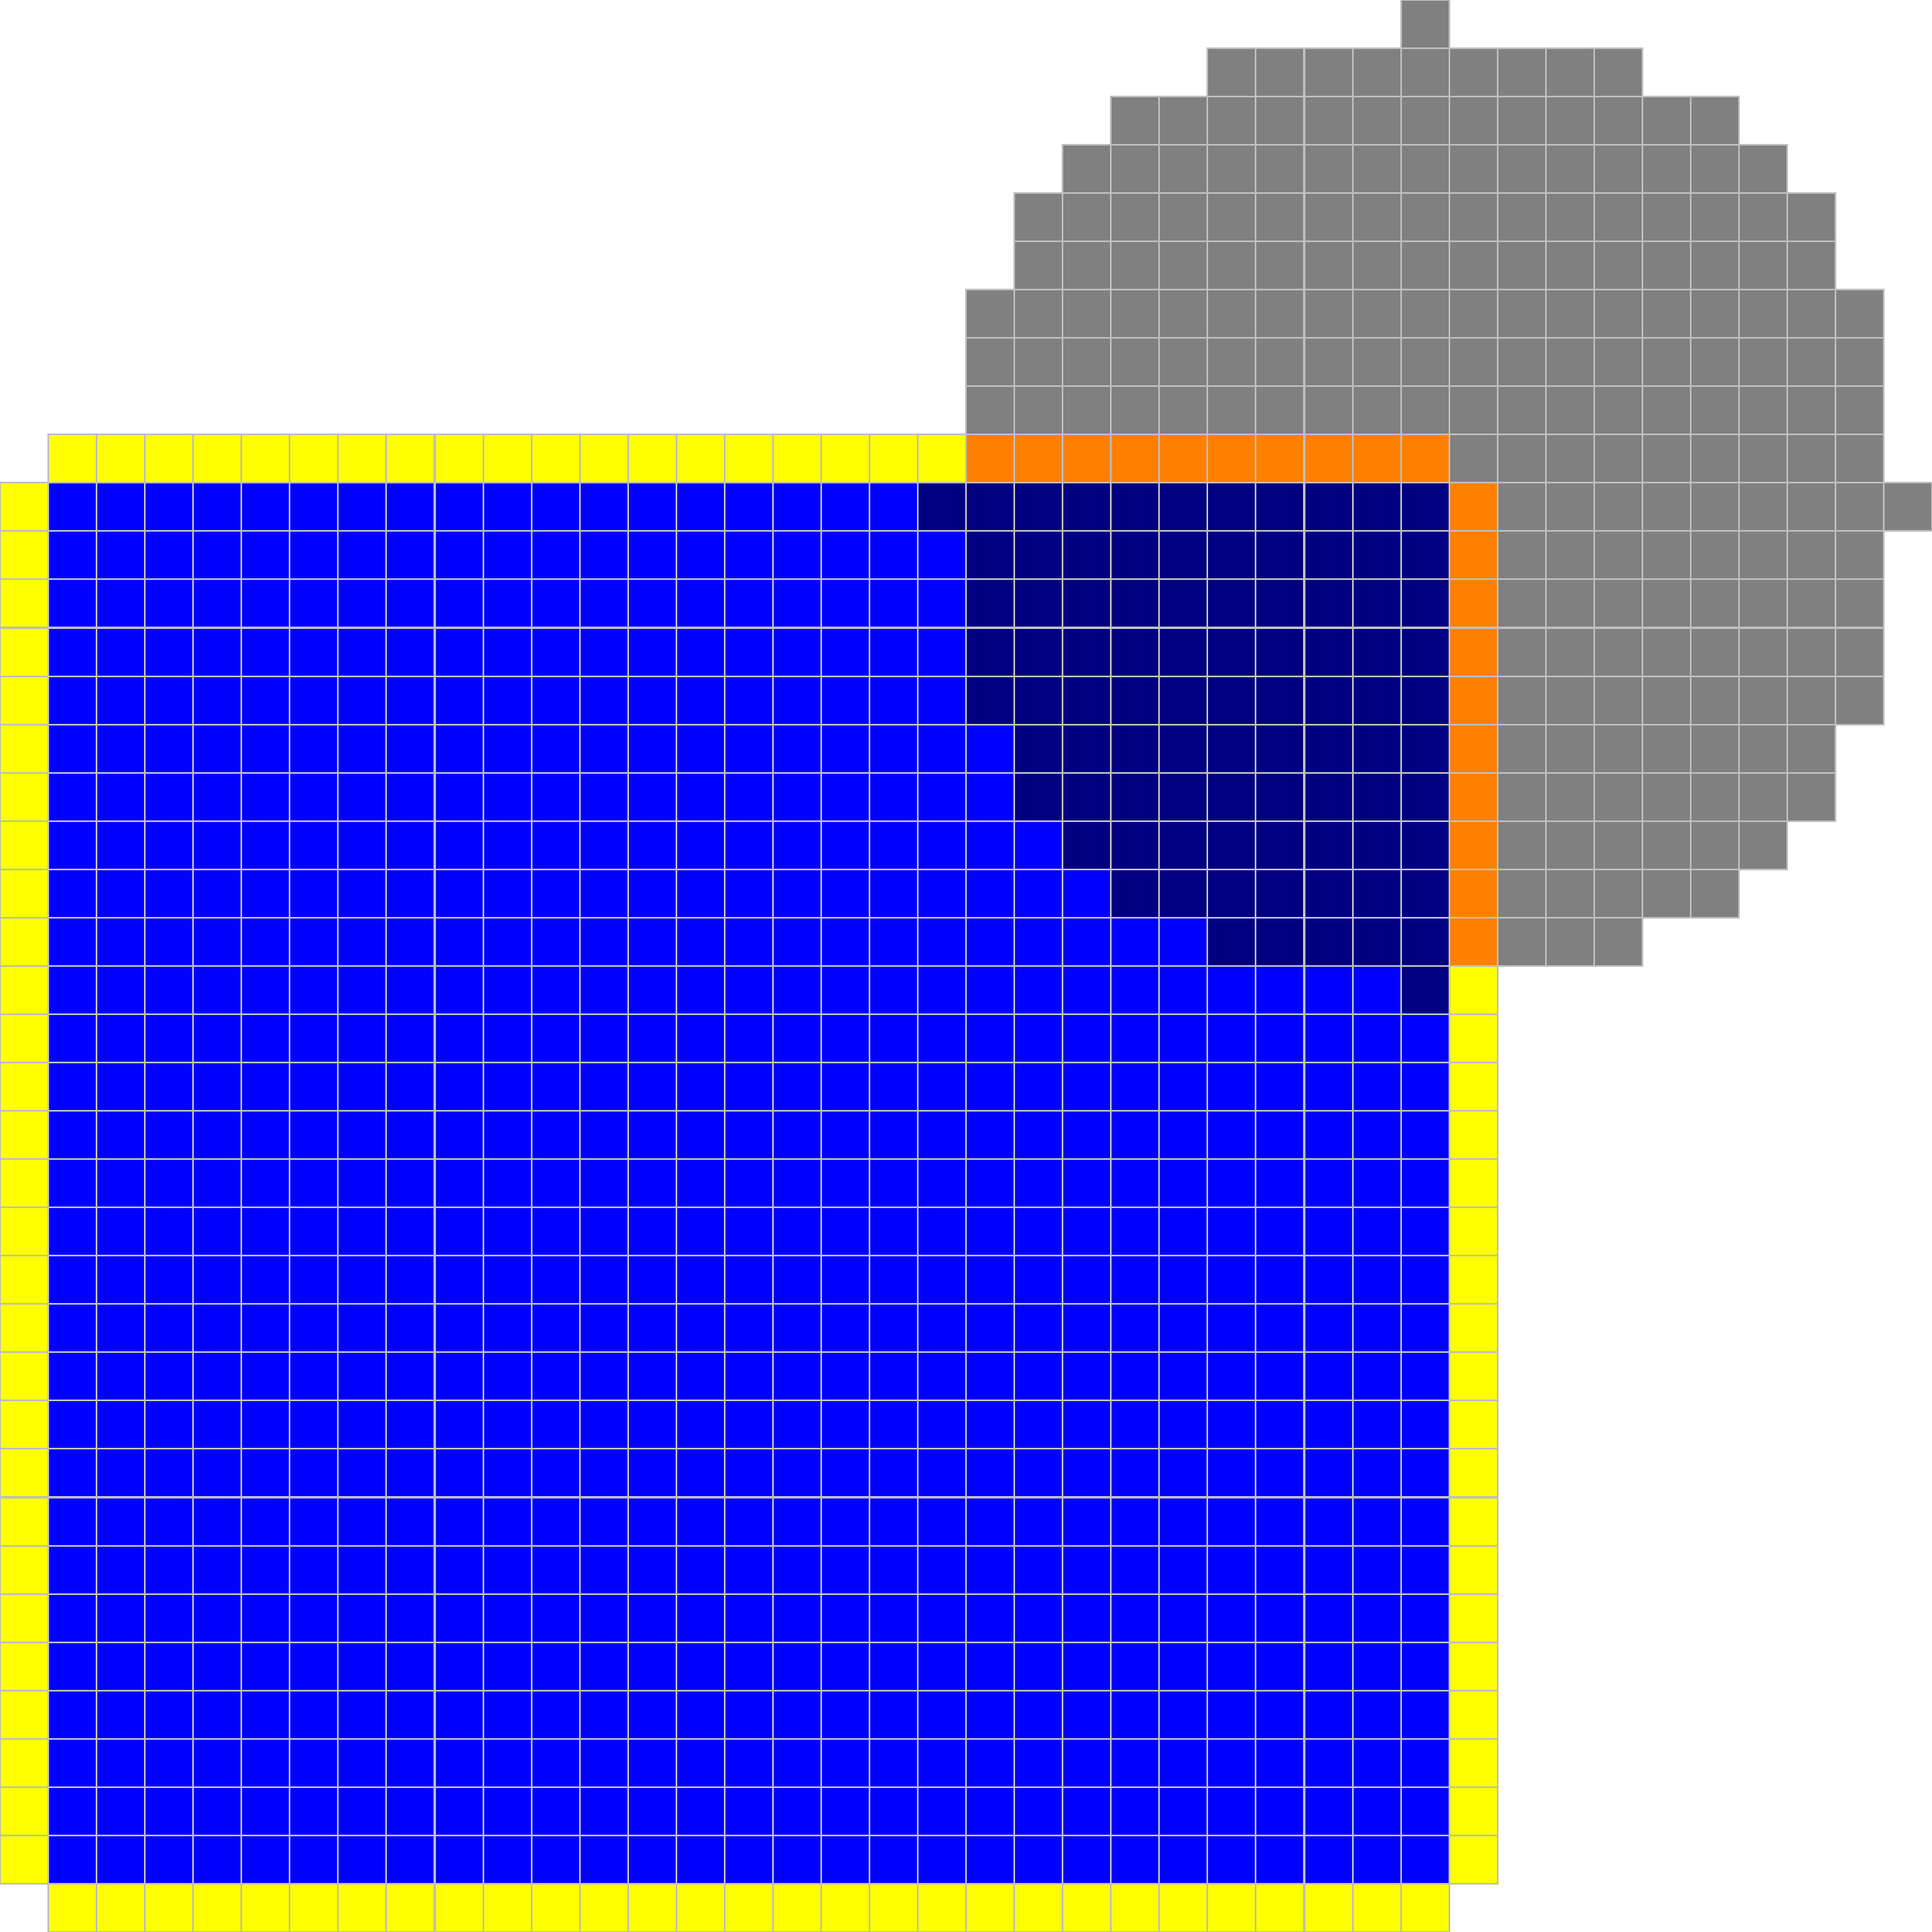
\includegraphics[scale=0.18]{figures/chapter6/contour-information/before-opt.pdf}}
\subfloat[\label{fig:naive-opt-after}]{

\includegraphics[scale=0.18]{figures/chapter6/contour-information/after-opt.pdf}}
\caption{Solution of model \eqref{eq:naive-opt-problem} for the square shape $(h=0.5,r=10)$. In (a) we have the square shape before minimization. Optimization variables are colored yellow. In (b), the resulting shape of the optimization problem. }
\label{fig:naive-opt-problem}
\end{figure}

The solution in figure \ref{fig:naive-opt-after} should not cause any surprise. The energy \eqref{eq:naive-opt-problem} is optimized over a fixed contour, i.e., independently of pixels being labeled zero or one, the estimation balls are evaluated at the same initial contour. In section \label{sec:global-optimization-model} we defined an optimization energy in which contour information is taken into account, but we end up with a difficult energy to optimize.

Nonetheless, we can exploit the II estimator definition to derive a energy which the minimization will lead to a shape with lower digital elastica value.


\begin{definition}{Balance coefficent}
Given digital shape $S \in \Omega$, positive number $r$ and point $p \in S$, the \emph{balance coefficient} of $S$ at $p$ is defined as

\begin{align*}
	u(p) = \left( \frac{\pi r^2}{2} - |B_r(p) \cap S| \right)^2.
\end{align*}

\end{definition}

The balance coefficient is a measure of how close an estimation ball is from estimating zero curvature. In figure \ref{fig:balance-plot}, we plot the balance coefficients of points in the diagonal of a square shape. 

\begin{figure}[h!]
\center
\begin{minipage}{0.25\textwidth}
\subfloat{
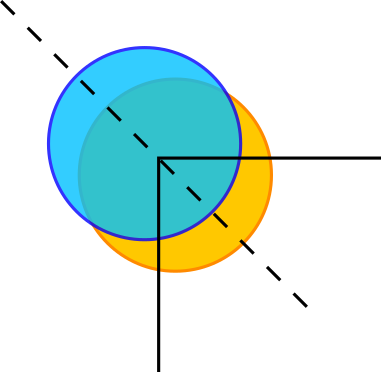
\includegraphics[scale=1.0]{figures/appendix-potential-elastica/distant-disks-1.png}}\\%
\subfloat{
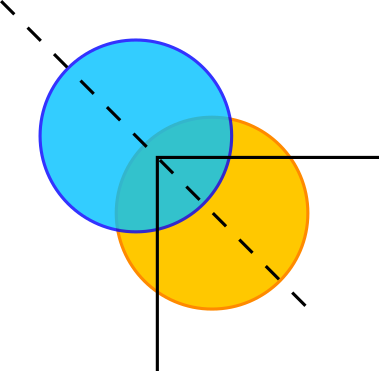
\includegraphics[scale=1.0]{figures/appendix-potential-elastica/distant-disks-2.png}}\\%
\subfloat{
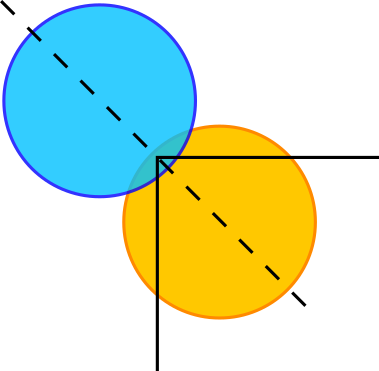
\includegraphics[scale=1.0]{figures/appendix-potential-elastica/distant-disks-3.png}}
\end{minipage}%
\begin{minipage}{0.75\textwidth}
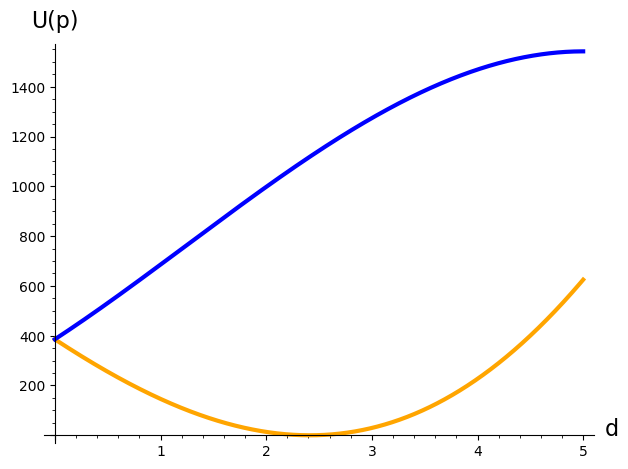
\includegraphics[scale=0.75]{figures/appendix-potential-elastica/potential-elastica-plot.png}
\end{minipage}
\caption{The balance difference of equidistant points from the shape contour preserves squared curvature information.}
\label{fig:balance-plot}
\end{figure}


We notice that the difference between outer and inner balance is non-negative along all the points in the diagonal. In fact, this is true for any point of positive curvature. For negative curvature, this difference is negative. This is the key observation for the definition of the digital flow.

\begin{definition}{k-potential}
Given digital shape $S$, natural numbers $r>0, k \neq 0$, the \emph{k-potential} at point $p$ is defined as

\begin{align*}
	U_{S,k}(p) &= \sum_{q \in Q(p)}{ u(q),}
\end{align*}

where its balance set $Q(p)$ is defined as

\begin{align*}
	\mathcal{Q}(p) &= \left\{\; q \; | \; q \in L_k(S),\; p \in B_r(q) \; \right\}.
\end{align*}

\end{definition}

\begin{figure}[h!]
\center
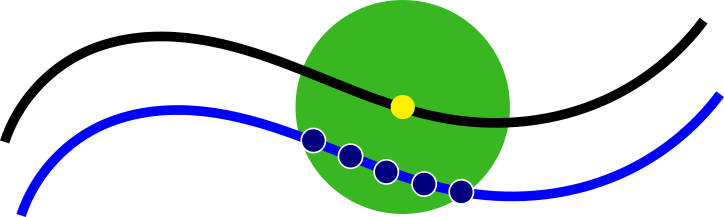
\includegraphics[scale=0.5]{figures/appendix-potential-elastica/k-potential.png}
\caption{The blue points forms the balance set of the yellow point.}
\label{fig:balance-set}
\end{figure}

The balance set of $p$ is the set of all points $q$ in which the $p$ is contained in the estimation ball centered at $q$.  In figure \ref{fig:balance-set} we illustrate the balance set definition. The k-potential is used to decide which pixels are to be removed or to be kept in the next shape of the flow. 


\begin{definition}{$k$-flow}
	Given digital shape $X$, let $\Delta U_{S,k}(p) = U_{S,k}(p) - U_{S,-k}(p)$. Then we define its $k$-flow as
	
	\begin{align*}
		F_k = \Big\{& S^{(i)} \; | \\
			& S^{(0)} = S,\\
		    &S^{(i+1)} = \argmin \sum_{ x_j \in X(I(S^{(i)}))}{ x_j \Delta _j\big(\; \Delta U_{S^ {(i)},k}(x_j) \;\big)} - \frac{x_j}{2}\sum_{ x_l \in X(I(S^{(i)}))}{x_l \Delta _{jl}\big(\; \Delta U_{S^ {(i)},k}(x_j) \;\big)} \; \Big\}.
	\end{align*}
     	  
\end{definition}	

\section{Balance plot development}
	The balance difference at a point $c \in S$ distant $d$ units from the corner is written as
	\begin{align*}
		u_i(c) &= \frac{\pi r^2}{2} - \big( \; a^2 + area( APC ) + area(A'PC) + area(\arc{PQ})  \; \big) \\
		&= \frac{\pi r^2}{2} - \big( \; a^2 + a(P_x-a) + \frac{\theta_P + \theta_Q + \pi/2}{2\pi} \pi r^2\; \big),
	\end{align*}
	
	where
	
	\[
	\begin{array}{ll}
	a = d\sqrt{1/2} & \theta_P = \arctan \frac{a}{P_x-a} \\		
	Q_y = -P_x = a + \sqrt{r^2 -a^2} & \theta_Q = \arctan \frac{a}{|Q_y|-a}		
	\end{array}\]
	
%default = pi*R^2*(abs(t2) + abs(phi))/(2*pi) + a*abs(p2[0])

%g2 = pi*R^2/2 - ( pi*R^2 - ( pi*R^2/4 - default) )	
	
	Similarly, for the outer ball
	\begin{align*}
		u_o(c) &= \frac{\pi r^2}{2} - \big(\; \frac{\pi r^2}{4} - area(APC) - area(AQC) - area(\arc{CP'}) - area(\arc{CQ'}) \; \big)\\
		&= \frac{\pi r^2}{2} - \big( \; \frac{\pi r^2}{4} - aP_x - \frac{\theta_P + \theta_Q}{2\pi}\pi r^2 \; \big),
	\end{align*}
	
	where
	\[
	\begin{array}{ll}
		a = d\sqrt{1/2} & \theta_P = \arctan \frac{a}{P_x+a}\\
		Q_y = -P_x = \sqrt{r^2-a^2} - a & \theta_Q = \arctan \frac{a}{|Q_y|+a}
	\end{array}	 \]
	
\begin{figure}[h!]
	\begin{minipage}{0.5\textwidth}
	\center
	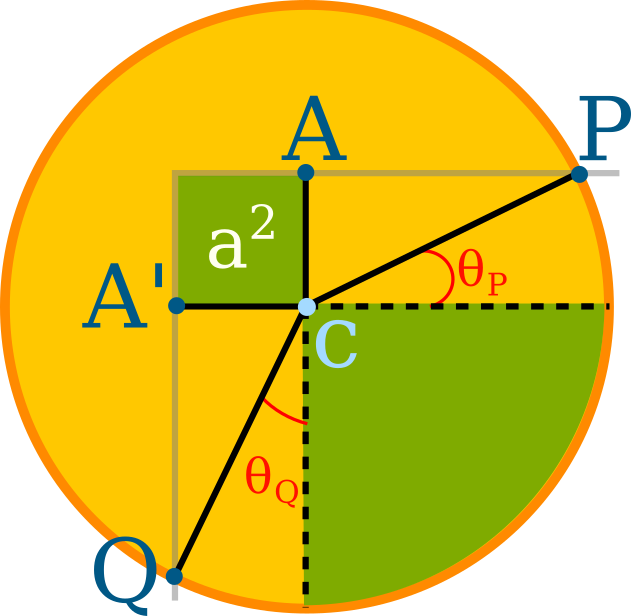
\includegraphics[scale=2.0]{figures/appendix-potential-elastica/balance-dev-1.png}
	\end{minipage}%
	\begin{minipage}{0.5\textwidth}
	\center
	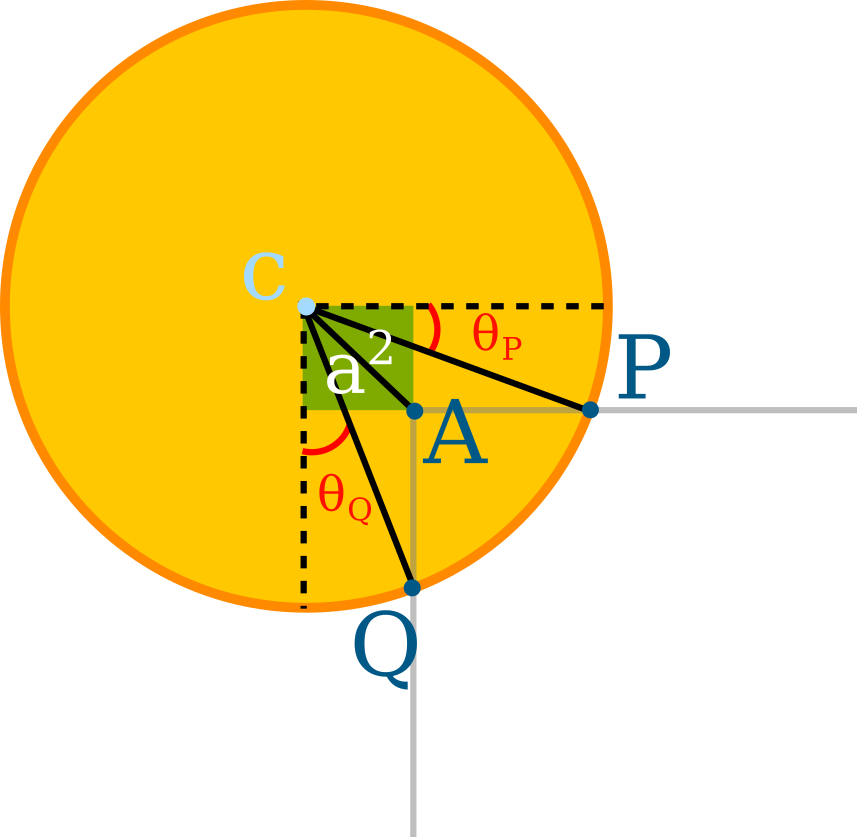
\includegraphics[scale=2.0]{figures/appendix-potential-elastica/balance-dev-2.png}
	\end{minipage}	
\end{figure}
